\chapter{多址接入系统分析}
\textbf{多址接入系统:}, 各用户拥有 不同的地址 ,互相 只能\textbf{通过公用
信道 联系},而不像传统的转接方式那样,用
户都集中到一个交换站,站线的线路只能作
为两个站之间的信道进行点对点的通信。这
类 公用信道的方式 ,称为 多址接入方式\\
特点:一条公用信道连接所有终端,按协议分配信道。\\
接入方法:
\begin{enumerate}
	\item 受控接入:
	\begin{itemize}
		\item 集中式控制
		\item 分散式控制
	\end{itemize}
	\item 随机接入:如ALOHA和CSMA/CD。
\end{enumerate}
\textbf{信道访问方式:}
\begin{figure}[H]
	\centering
	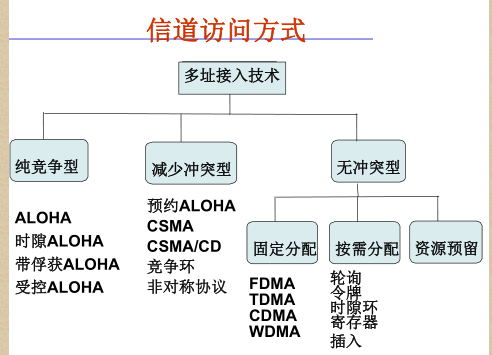
\includegraphics[width=0.7\linewidth]{figures/screenshot001}
	\caption{}
	\label{fig:screenshot001}
\end{figure}
\section{纯ALOHA系统}
\subsubsection{纯ALOHA基础}
定义:系统发包想发就发,如冲突,等待随机时间后重发。(信息包的长度P = 发送一个包所需的时间,即服务时间$ \tau $)
\begin{figure}[H]
	\centering
	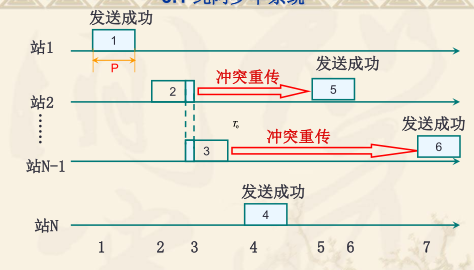
\includegraphics[width=0.7\linewidth]{figures/screenshot002}
	\caption{}
	\label{fig:screenshot002}
\end{figure}
特点:
\begin{enumerate}
	\item 以定长信息包的方式发送到信道,随机方式抢占信道
	\item 如有碰撞,之后随机地重发。
\end{enumerate}
要想发送不碰撞,发包前P时间和发包后P时间即从t-P到t+P时间内没有其他站发包。
\begin{figure}
	\centering
	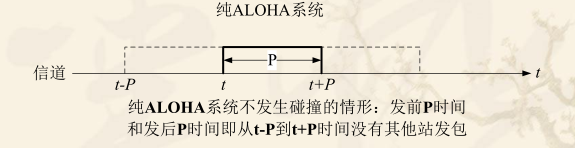
\includegraphics[width=0.7\linewidth]{figures/screenshot003}
	\caption{}
	\label{fig:screenshot003}
\end{figure}
\subsubsection{系统通过量}
\begin{itemize}
	\item  设有无限个用户公用一个信道,这些用户
	的总呼叫是以$ \lambda $为均值的泊松流
	\item 每个发包定长为P,亦即服务时间$ \tau $,所以系统的呼叫量$ a = \lambda \tau = \lambda P$。令P=1,则$ \lambda = a $,所以t内有r个呼叫或信息包发上信道的概率为
	\begin{equation}\label{key}
	p_r = \frac{(\lambda t)^r}{r!}e^{-\lambda t} = \frac{(a t)^r}{r!}e^{-a t}
	\end{equation}
	则t时间内没有包发送的概率为
	\begin{equation}\label{eq:1}
	p_0 = e^{-\lambda t} = e^{-at}
	\end{equation}
	要想成功发送一个信息包即在2P时间段内没有其他包发送,$ t = 2P,P = 1 $(也可通过$ \lambda = a/P$得到)。带入\ref{eq:1},有成功发送包的概率为
	\begin{equation}\label{key}
	p_0 = e^{-2a}
	\end{equation}
	所以发送信息包失败的概率为:
	\begin{equation}\label{key}
	p = 1-p_0 = 1- e^{-2a}
	\end{equation}
\end{itemize}
通过量定义为:平均成功的信息包
所占的时间与总观察时间之比.当信息包
长1 时,这就是单位时间成功的信息包数
\begin{equation}\label{key}
y = ae^{-2a}
\end{equation}
a = 0.5时,ymax = 0.184,纯阿罗华系统效率低下,重发频繁,系统不稳定。
\subsection{下一个2t时刻系统存包量讨论}
 假设增加 假设增加i 个,求条件概率p(i|k) ,其中i=-1,
0, 1, 2, …  ;i=-1相当于减少一个旧包。 相当于减少一个旧包。
A
\begin{figure}[H]
	\centering
	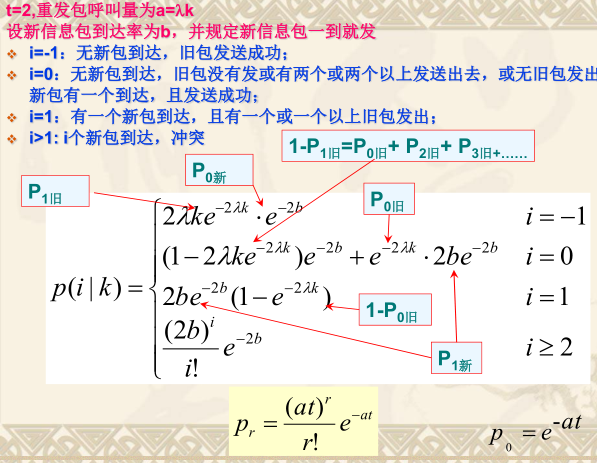
\includegraphics[width=0.7\linewidth]{figures/screenshot004}
	\caption{}
	\label{fig:screenshot004}
\end{figure}
最后可得期望
\[ 
E(i|k) = \sum_{i=-1}^{\inf}ip = 2b - 2(b+\lambda k)e^{-2(b+\lambda k)}
 \]
\begin{itemize}
	\item 当E$ \ge $ 0时,系统不是稳定的.
	\item 当E<0时,系统稳定
	\item 当$ b+\lambda k = 0.5 $达到最小值$ 2b -e^{-1} = 2b - 0.368 $
	\begin{itemize}
		\item b>0.184,系统不稳定
	\end{itemize}
\end{itemize}
解开结的办法:
\begin{enumerate}
	\item b = 0,不让新包进入
	\item 调整旧包重发率,旧包重发率$ \lambda $ ,以使k虽大, 
	而$ \lambda $还是较小的,而且最好能使 $ b+\lambda k=0.5 $ 还是较小的,而且最好能使
	$ b+\lambda k=0.5 $ ,以使E(i|k)最小,尽快解 最小,尽快解
	开这个结。当然此时 开这个结。当然此时b 必须小于0.184
\end{enumerate}
\section{分槽阿罗华系统(时隙ALOHA,S-ALOHA)}
各站时间同步, 所有用户都与主时钟同步,时隙(slot) 的长度: 信息包长度 p= 一帧的长度$ T_0 $
• 在\textbf{每一个时隙的开始时才发送数据}, 冲突后的重发策略
与纯ALOHA 的情况相似。
• 帧能够发送成功条件是 \textbf{没有其他帧在同一时隙内A} 达到
\begin{figure}[htbp]
	\centering
	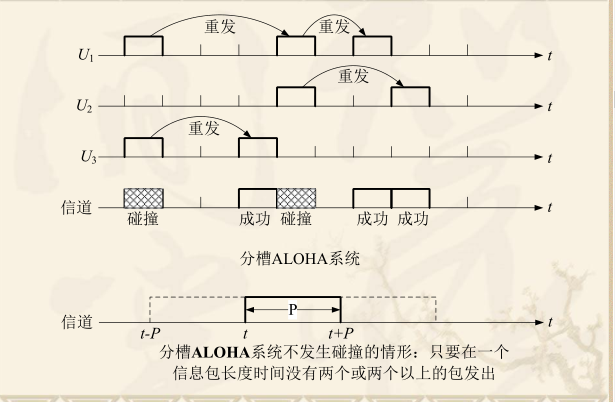
\includegraphics[width=0.7\linewidth]{figures/screenshot005}
	\caption{}
	\label{fig:screenshot005}
\end{figure}
所以,发送一个包成功的概率:
\begin{equation}\label{key}
p_0 = e^{-a}
\end{equation}
碰撞的概率:
\begin{equation}\label{key}
p = 1-p_0 = 1-e^{-a}
\end{equation}
系统的通过量:
\begin{equation}\label{key}
y = ae^{-a}
\end{equation}
当a=1时,ymax=0.368,通过量较纯ALOHA系统提高了一倍,这种提高使以\textbf{全网同步控制为代价}而获得的。
\subsection{两个系统的比较}
\begin{figure}[H]
	\centering
	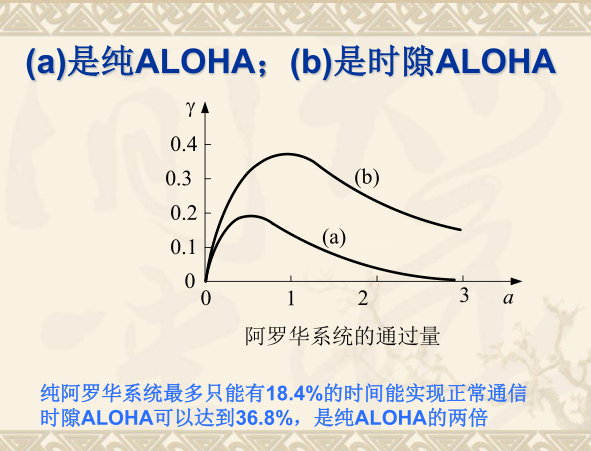
\includegraphics[width=0.7\linewidth]{figures/screenshot006}
	\caption{}
	\label{fig:screenshot006}
\end{figure}
\subsection{碰撞重发的稳定性}
\begin{figure}[H]
	\centering
	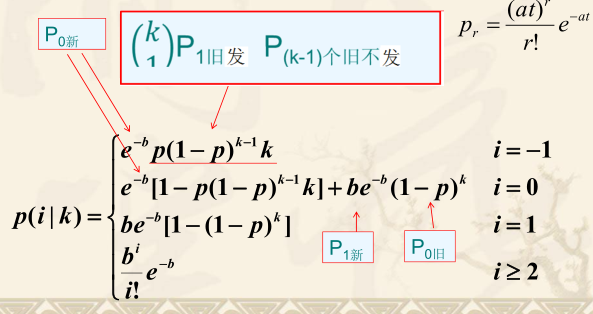
\includegraphics[width=0.7\linewidth]{figures/screenshot008}
	\caption{}
	\label{fig:screenshot008}
\end{figure}
最后可得期望
\[ 
E(i|k) = \sum_{i=-1}^{\inf}ip = b - e^{-b}(1-p)^{k-1}[b+(k-b)p]
\]
经过求导,当$ p = \frac{1-b}{k-b} $时,E = b-0.368。
即,b大于最大通过量时,系统不是稳定的。有效的控制策略时,k相当大后,令b=0,不让新包进入。
\section{载波监听多址接入系统}
波监听多址接入( 载波监听多址接入(CSMA)是阿罗华系统的一 )是阿罗华系统的一
种改进形式,适用于延时较小的总线网。\\
 总线网上每个用户节点都设有\textbf{载波 监听} 装置,以
接收到载波与否来判断线路上的忙闲状态。用户
只能在总线空闲时启动发送一个信息包\\
监听方式分类:
\begin{itemize}
	\item 坚持监听CSMA-P,监听装置一直连续在监听,一旦
	发现信道空闲就发出信息包( 发现信道空闲就发出信息包(1- 坚持CSMA)或者以 )或者以
	一定概率发送信息包( 一定概率发送信息包(P- 坚持CSMA)。
	\item 非坚持监听CSMA-NP,监听装置听到 ,监听装置听到 忙状态后,停
	止监听, 再过一个随机时间才再次监听,直到有空再
	发信息包。
\end{itemize}
\subsection{传播时延对载波监听的影响}
\textbf{当某个站听到总线时空闲时,也可能总线并非真正时空闲的}
\begin{figure}[htbp]
	\centering
	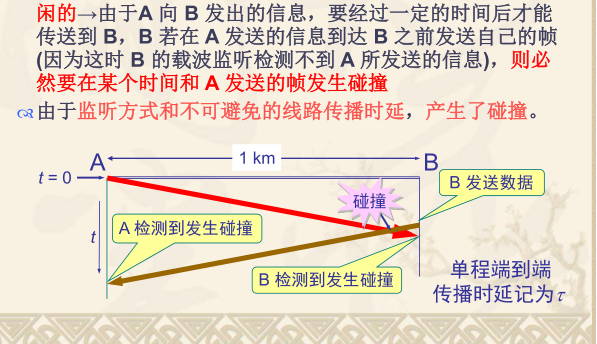
\includegraphics[width=0.7\linewidth]{figures/screenshot009}
	\caption{}
	\label{fig:screenshot009}
\end{figure}
CSMA-CD:发送数据前监听信道,信道一旦空闲立即发送数据,便发送数据边监听信道(进行冲突检测)。该方式为完全分散控制方式。
\subsection{非坚持监听方式}
特点:
\begin{enumerate}
	\item 信道空闲,立即发送
	\item 一旦忙期,等待随机时间t再监听
	\item 碰撞主要由创博时延$ \epsilon $引起。
\end{enumerate}
\subsubsection{假设$ \epsilon $为0,则发包必然成功。有:}
\begin{itemize}
	\item 假设忙期:$ T_B = 1 $。
	\item 监听率为a(新包和旧包合起来的到达率为a),则平均空闲时长为$ T_I = \frac{1}{a} $,即两个包发送的间隔时间。
	\item 忙闲周期$  T_B + T_I = 1+\frac{1}{a} $,在整个时间周期内只有一个包发送,则信道的利用率或通过率为$ r=\frac{1}{1+\frac{1}{A}}  = \frac{a}{1+a}$
\end{itemize}
\subsubsection{假设$ \epsilon $不为0。有:}
\begin{figure}
	\centering
	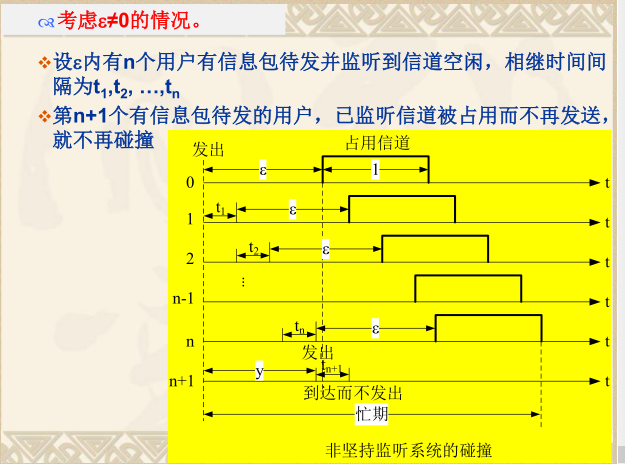
\includegraphics[width=0.7\linewidth]{figures/screenshot010}
	\caption{}
	\label{fig:screenshot010}
\end{figure}
满足:
\begin{gather}
y = t_1+t_2+\dots+t_n \\
y<\epsilon \\
y+t_{n+1} > \epsilon
\end{gather}
y的均值为
\begin{equation}\label{key}
y = \epsilon - \frac{1}{a}(1-e^{-\epsilon a})
\end{equation}
平均忙期为y+$ \epsilon $+1.(最后一个包发送的时刻+时延+一个包的长度)
平均忙闲周期为
\begin{equation}\label{key}
y+\epsilon +1 + \frac{1}{a}
\end{equation}
\begin{figure}[H]
	\centering
	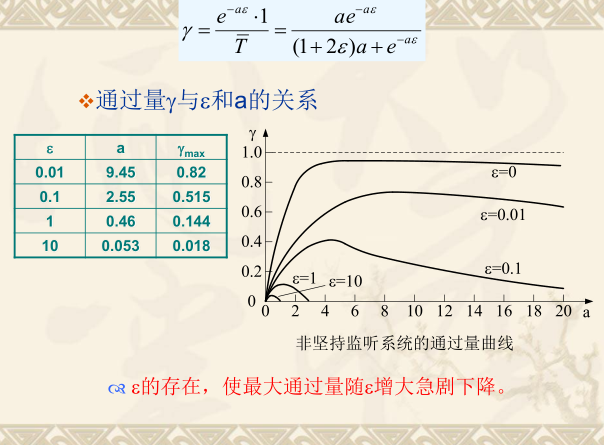
\includegraphics[width=0.7\linewidth]{figures/screenshot011}
	\caption{}
	\label{fig:screenshot011}
\end{figure}
\subsection{坚持监听方式}
此时用户一直监听信道的状态,监听到信
道空闲,且有通信要求,就发送信息包。
显然,若两个以上用户同时有新包待发,
必发生碰撞。传播时延愈大,碰撞的机会
愈大。\\
\subsubsection{假设$\epsilon$为0的情况}
\begin{gather}
p_n = (1-e^{-a})^{n-1}e^{-a}
\end{gather}
前n-1个信息包,有一个或一个以上待发,第n个信息包必无信息包待发。则,忙期的平均长度为:
\begin{equation}\label{key}
T_B = \sum_{n=1}^{\inf}np_n = e^a
\end{equation}
 平均忙闲周期为:\begin{equation}\label{key}
 T = T_I+T_B = \frac{1}{a}+e^a
 \end{equation}
 每个信息包成功发送的概率:
 \begin{equation}\label{key}
 p = \frac{ae^{-a}}{1-e^{-a}}
 \end{equation}
 分子时出现一个呼叫的概率,分母是出现呼叫的概率,但排除了不出现呼叫的情况。\\
 
 一个忙期内平均成功的包数为:
 \begin{equation}\label{key}
  1+a
 \end{equation}
\begin{figure}[H]
	\centering
	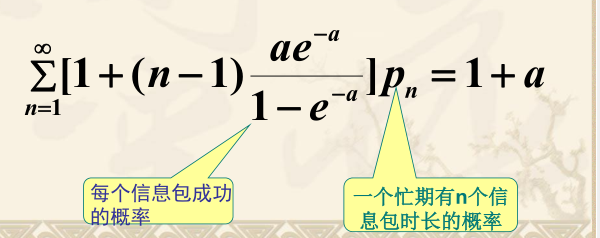
\includegraphics[width=0.7\linewidth]{figures/screenshot012}
	\caption{}
	\label{fig:screenshot012}
\end{figure}
通过量为:
\begin{equation}\label{key}
y = \frac{1+a}{T} = \frac{a(1+a)}{1+ae^a}
\end{equation}
当a=1.03,ymax = 0.54,当a>1.03时,系统将不稳定。
\subsubsection{假设$ \epsilon $不为0时}
\begin{description}
	\item[第一类时段] 紧接在闲期后面的一个信息包并包括碰撞和延时这一段。当一个信息包发出后,$ \epsilon $内无其它信息包代发,这个信息包就发送成功,其概率为 \begin{equation}\label{key}
	 p_1 = e^{-a\epsilon}
	\end{equation}。如果有其他包在$ \epsilon $这段时间到达,则会发生碰撞。这种情况和非坚持监听一样,其平均忙期时长为:
	\begin{equation}\label{key}
	T_1 = y+1+\epsilon
	\end{equation}
	\item [第二类时段] 紧接在第一类时段或第二类时段之后出现的忙期,在第二类时段内首先发出的信息包成功的概率是起始的$ \epsilon $内无信息报,而前段中后面的1+$ \epsilon $内有且只有一个信息包,这概率为:
	\begin{equation}\label{key}
	p_2 = e^{-a\epsilon}\frac{a(1+\epsilon)e^{-a(1+\epsilon)}}{1-e^{-a(1+\epsilon)}}
	\end{equation}
	这两类时段内平均长度与$ T_1 $一样。即$ T_2 = T_1 $
\end{description}
经过转移矩阵求得各状态概率0,1,2。求出平均成功的发包数量,最后推出通过量为
\begin{equation}\label{key}
y = \frac{a(1+a+a\epsilon)e^{-a(1+2\epsilon)}}{e^{-a\epsilon}+e^{-a(1+\epsilon)+a+2a\epsilon-1}}
\end{equation}
\subsubsection{通过量y与$ \epsilon $h和a的关系}
\begin{figure}[H]
	\centering
	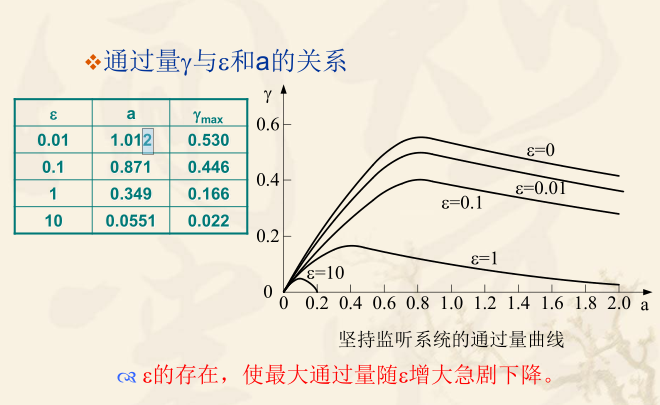
\includegraphics[width=0.7\linewidth]{screenshot001}
	\caption{}
	\label{fig:screenshot001}
\end{figure}
\subsection{监听检测方式}
为了提高信道利用率,可采用 碰撞检测 。每当发
出信息包后就检测是否与别的用户所发的信息包
发生碰撞。一旦发现碰撞,立刻停止发送,以使
信道不致无效地继续被占用。\\
闲期和之前相同。忙期有两类:重点,应该会考。
\begin{itemize}
	\item 成功发送一个信息包,即一
	个信息包发出后,时延$ \epsilon $内无其他用户发出信息包,其概率为$ p_1=e^{-a\epsilon} $,这类时段的长度为$ T_1 = 1+\epsilon $。
	\item 有碰撞的情况,发送不成功。即在$ \epsilon $内有其他包发送。概率为$ p_2 = 1 - e^{-a\epsilon} $,这类时段的平均长度为$ T_2 = 2\epsilon + \overline{t} $。t为第一、第二个信息包之间的间隔时间。
\end{itemize}
非坚持监听,忙期不会连续出现,\textbf{一忙一闲}构成一个周期。
\begin{equation}\label{key}
T = T_0 + T_1p_1 + T_2p_2
\end{equation}
通过量:
\begin{figure}[H]
	\centering
	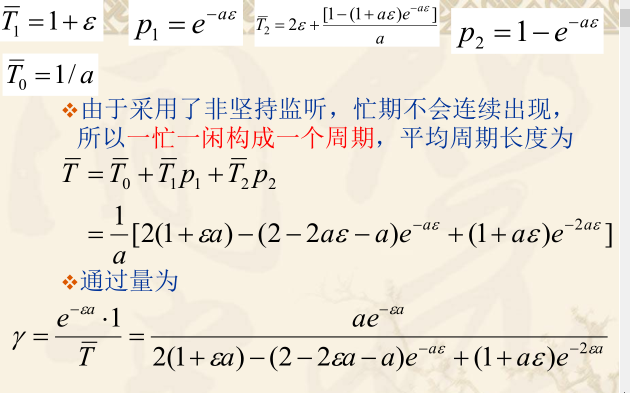
\includegraphics[width=0.7\linewidth]{figures/screenshot013}
	\caption{}
	\label{fig:screenshot013}
\end{figure}
\subsection{载波监听总结}
\begin{itemize}
	\item 随着时延增大,最大通过量急剧减小
	\item 从最大通过量来看,有碰撞检测的方式比没有的好。
\end{itemize}
\begin{figure}[H]
	\centering
	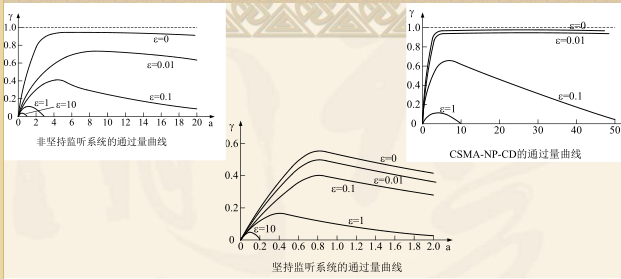
\includegraphics[width=1\linewidth]{figures/screenshot014}
	\caption{}
	\label{fig:screenshot014}
\end{figure}
\section{轮询方式 }
询( 轮询(Polling)方式是一种设有 )方式是一种设有 主站 的集
中 \textbf{控制、非竞争} 的方式
询问方式分类:
\begin{itemize}
	\item 依次轮询,可设置优先级。
	\item 传递轮询,不设置优先级,常用于环状网,子站收到后依次向后传递。
\end{itemize}
设$ b = P+2\epsilon + E $,有包发送的长度为1+b,无包发送的长度为b。
通过量:
\begin{equation}\label{key}
y = \frac{p}{b+p}
\end{equation}
p时每个子站有信息包发送的概率。\\
呼叫量与通过量的关系
\begin{equation}\label{key}
a = -\frac{1-y}{b}ln(1-\frac{by}{1-y})
\end{equation}
\begin{figure}[H]
	\centering
	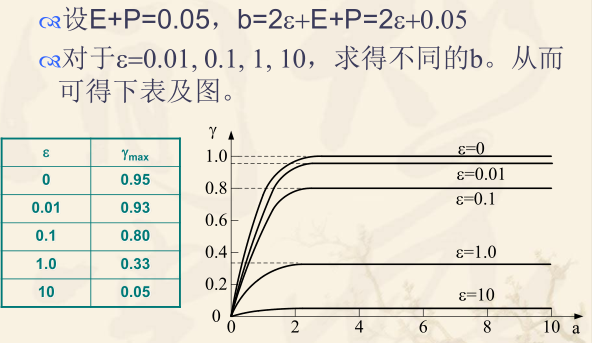
\includegraphics[width=0.7\linewidth]{figures/screenshot015}
	\caption{}
	\label{fig:screenshot015}
\end{figure}
\section{各种多址系统的比较}
\subsection{通过量}
当总呼叫率a很小的时候,通过量的比较:
\begin{description}
	\item[ALOHA] a(1-2a),原$ ae^{-2a} $
	\item[S-ALOHA] a(1-a),原$ a^{-a} $
	\item[CSMA-NP] $ a(1-(1+2\epsilon)a) $ 
	\item[CSMA-P] $ a(1-\epsilon a) $
	\item[CSMA-NP-CD] $ a(1-\epsilon a) $
	\item[Polling] $ y = a(1-\frac{b}{2}a) $
\end{description}
在a很小时,上述各种方法具有基本上相同的通过量a。只有与$ a^2 $成比例的一些呼叫中,未能利用信道
\begin{itemize}
	\item 阿罗华中,这一部分是由碰撞引起的。
	\item 载波监听中,除碰撞还有监听到信道被占用而放弃传送的。
	\item 在轮询方式中,由控制信令P和结束符E以及时延占用所致。
\end{itemize}
考察各项性能:(在a较小时)
\begin{itemize}
	\item 时延较小时,CSMA-P和CSMA-NP-CD,性能最好。轮询中有P和E,所以不算很好。
	\item 时延较大,以S-ALOHA最好,因为它与$ \epsilon $无关。
\end{itemize}
这样看来,\textbf{a较小时轮询方式并不是最优的},也就是从效果
来看,\textbf{碰撞的存在,并不是一个问题}。\\
a->$ \inf $时。
\begin{itemize}
	\item 所有有竞争的方式,只要有时延存在,都将使通过量趋于零。
	\item 对于中央空hi的非竞争 型的轮询方式,则将达到最大通过量。
\end{itemize}
\begin{figure}[H]
	\centering
	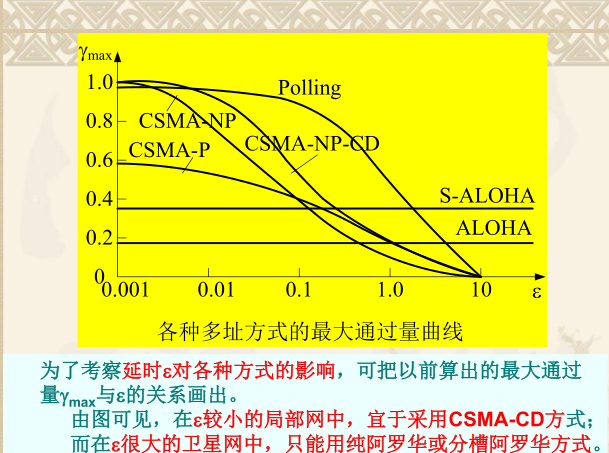
\includegraphics[width=0.7\linewidth]{figures/screenshot016}
	\caption{}
	\label{fig:screenshot016}
\end{figure}
\subsection{等待时间比较}
\subsubsection{轮询}
\begin{figure}[H]
	\centering
	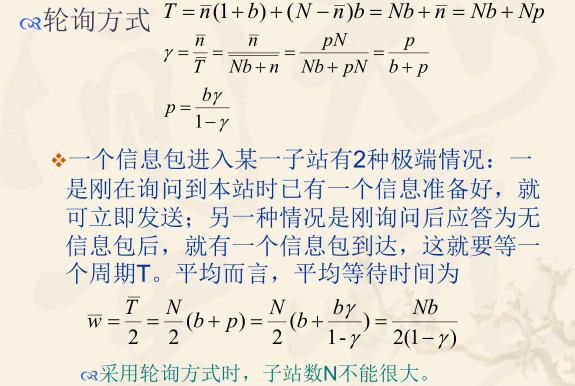
\includegraphics[width=0.7\linewidth]{figures/screenshot017}
	\caption{}
	\label{fig:screenshot017}
\end{figure}
\subsubsection{竞争型}
\begin{figure}[H]
	\centering
	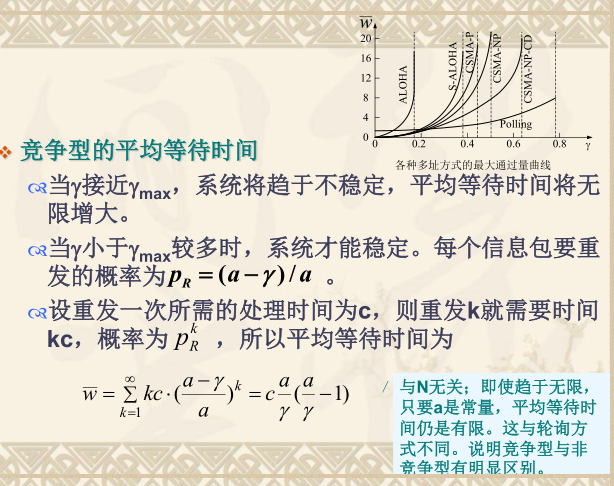
\includegraphics[width=0.7\linewidth]{figures/screenshot018}
	\caption{}
	\label{fig:screenshot018}
\end{figure}
上述表明,碰撞并不十分可怕,非竞争型并不一定好。各种
方式各有适用环境









